\section{Application Scenarios}
\label{sec:caseStudy}
% \shusen{A full case study that driven by the visualization task and the question associated with them}
%In this section, we discuss application scenarios, in which the domain experts utilize the 
To better illustrate how the proposed perturbation-driven exploration tool helps researchers interpret the neural network model, we present five application scenarios gathered by the domain experts who integrated the proposed tool into their analysis workflow.

\begin{figure}[htbp]
\centering
%\vspace{-2mm}
 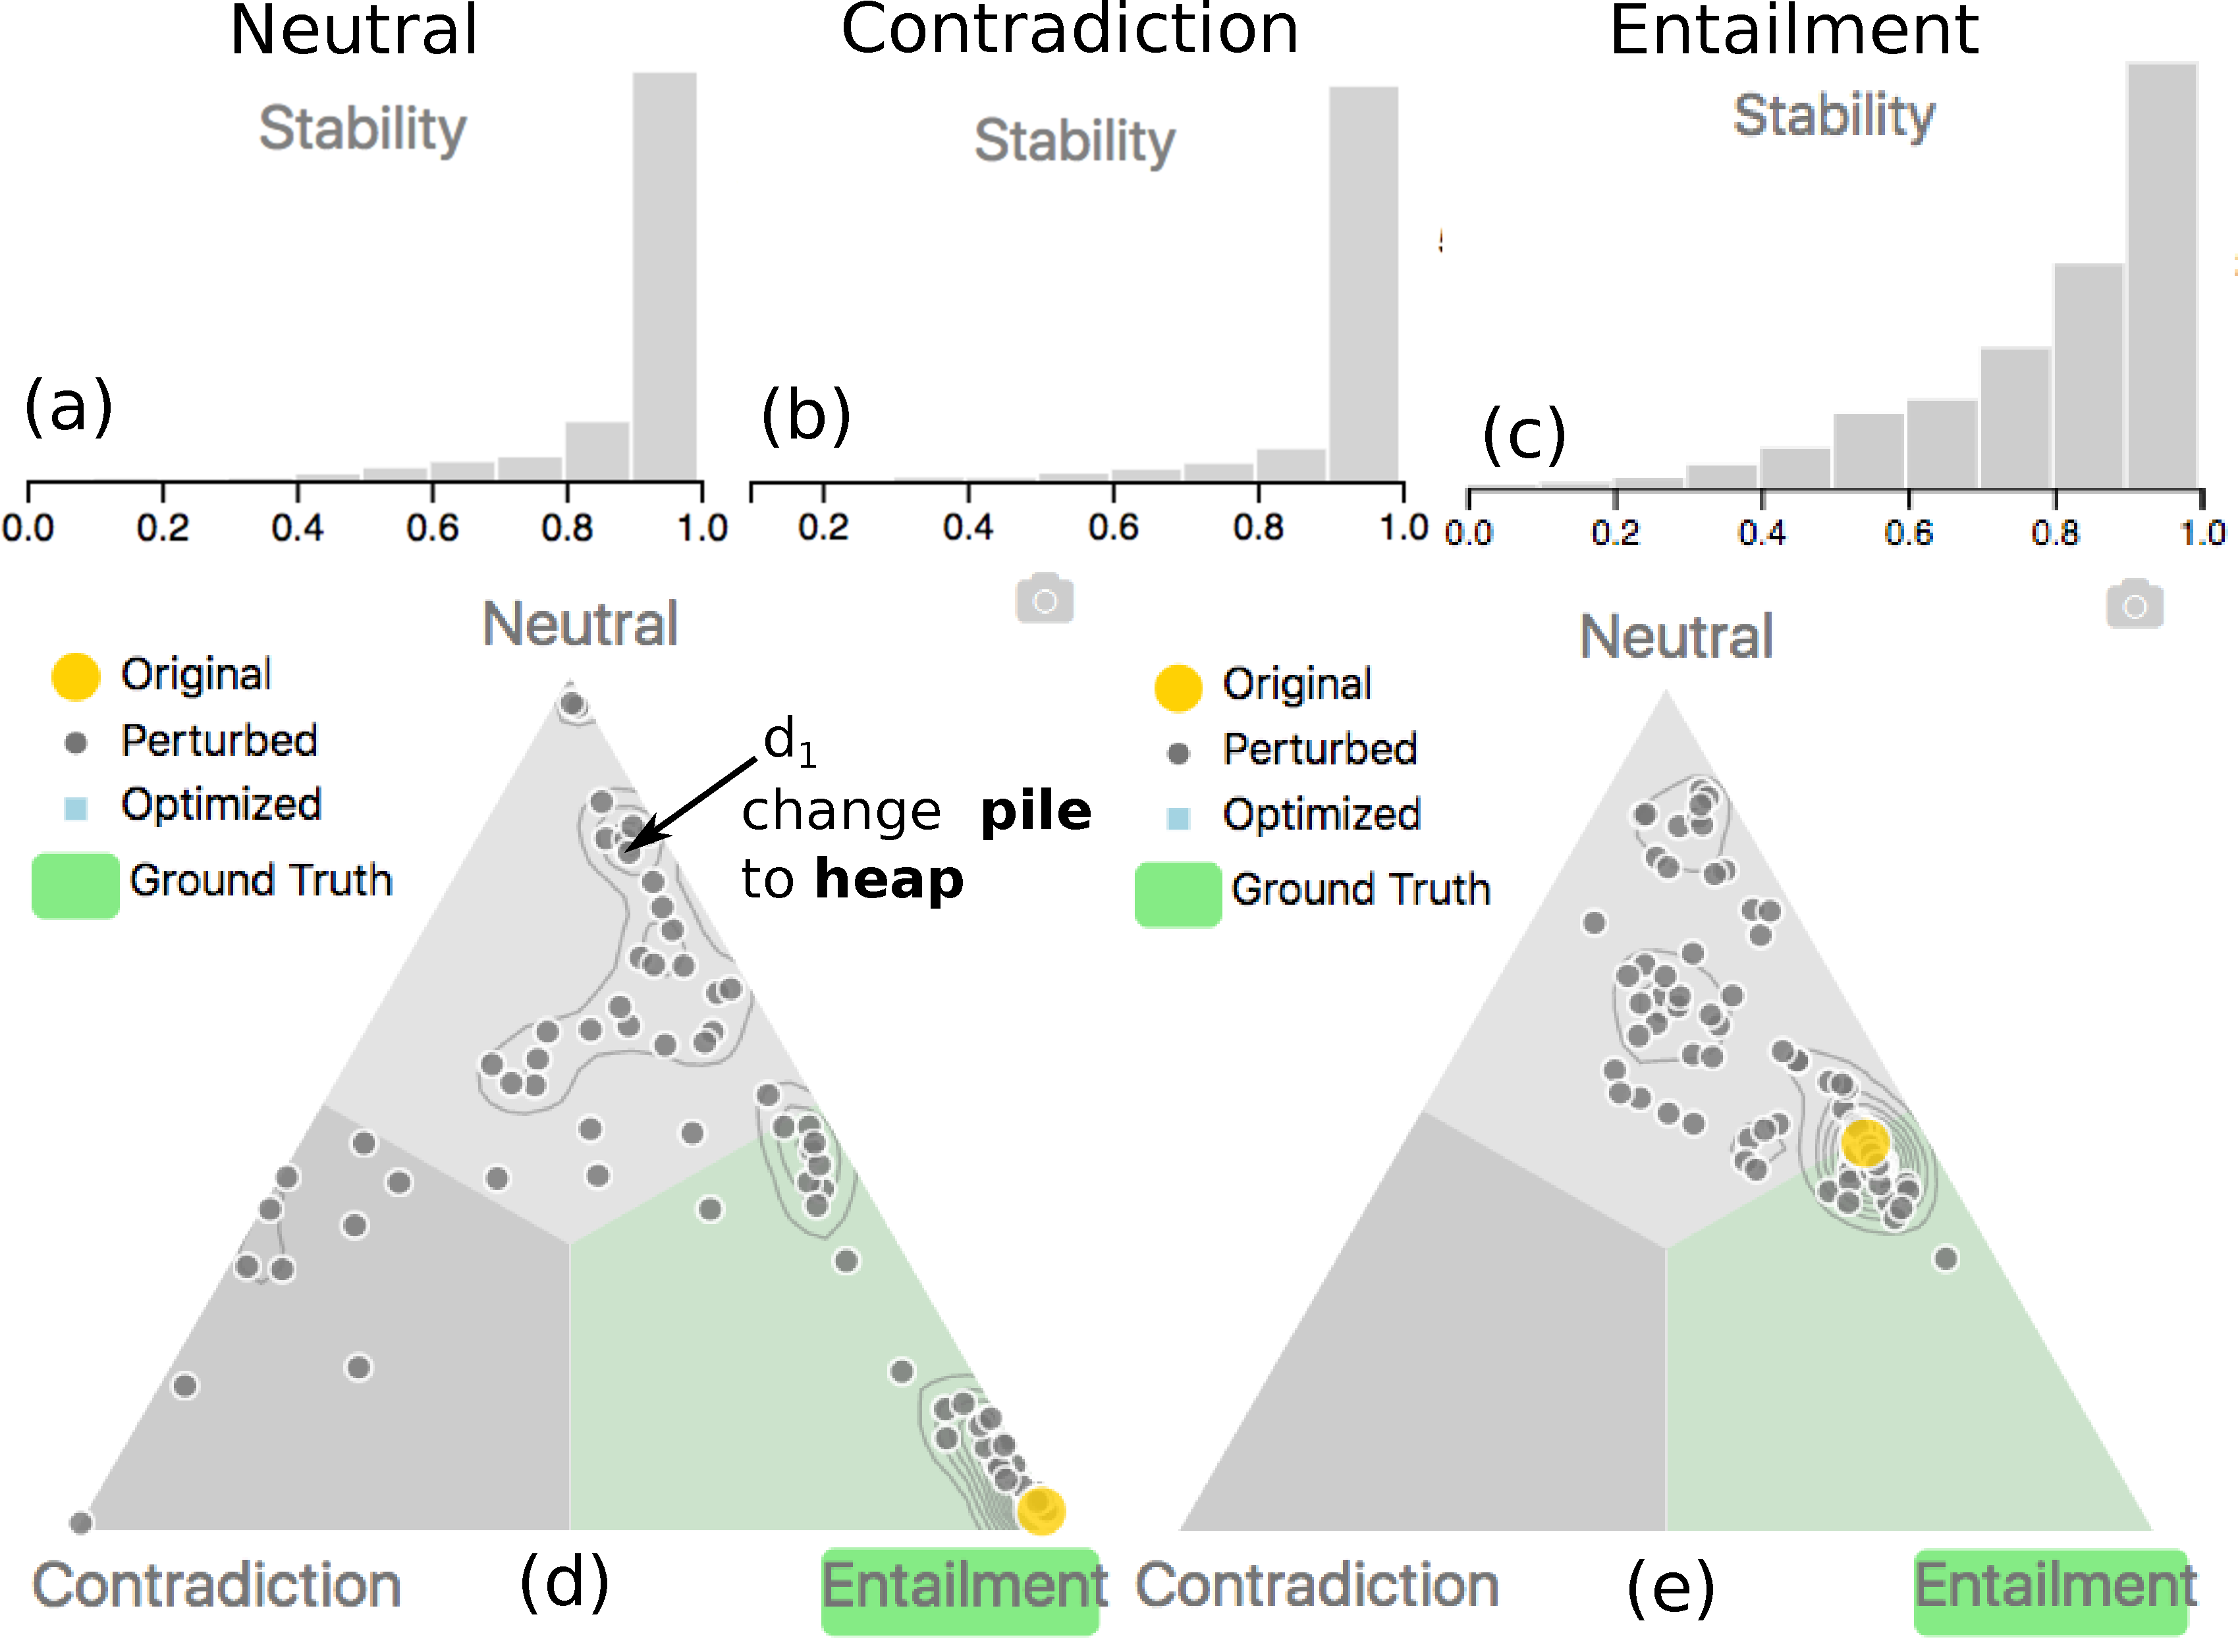
\includegraphics[width=1.0\linewidth]{predictStability}
 \caption{
Prediction stability assessment. In (a)(b)(c), we estimate the overall prediction stability (regarding synonymous perturbation) for each type prediction over the entire development set (10k examples). The user can drill down to individual examples by filtering via the histogram and scatterplot (see Fig.~\ref{fig:summaryView}) for a case by case exploration, as illustrated in (d)(e). For highly unstable outliers, we often observe the prediction of the original sentences near the decision boundary (e.g., the yellow circle in (f) corresponds to a entailment prediction that is very close to neural), however, some predictions, such as the one illustrated in (d) can alter the prediction quite drastically with minor perturbation (illustrated in $d_1$, where the word ``heap'' is replace by ``pile'' in the hypothesis sentence).
%
}
\label{fig:predictStability}
\end{figure}

\subsection{Scenario 1: Assess the Model Prediction Stability}
The robustness of the prediction is often hard to evaluate, however, they provide valuable information for the researchers to evaluate the model.
%
In the proposed work, we approach the prediction robustness from sensitivity analysis point of view. The stability of the prediction is measured by how often the predicted labels are altered after small perturbations are applied to the input. 
%
Compare to other types of input (e.g., image), perturbation of the natural language can be particular tricky, as small alteration of words can drastically change the meaning of the sentence. As discussed in Section~\ref{sec:sentence}, we try to maintain semantic of the sentence by only replace words with their synonymous and only replace one word for each pair.
%
As illustrated in Fig.~\ref{fig:predictStability}, by utilizing the automated input perturbation and visual interface in the proposed tool, the domain expert can not only examine visual summary of the stability, but also quickly dive into individual examples for case by case analysis.%which system input sentence perturbation to assess the overall stability of the prediction. 

By viewing the distribution of the stability in the histogram (Fig.~\ref{fig:predictStability}(a)(b)(c)), we estimate the overall prediction stability (regarding synonymous perturbation) for each type prediction over the entire development set (10k examples).
%
We can observe a drastic difference between the stability for entailment predictions compare to the contradiction and neutral ones.
%
Such a distinction can be partially explained by how entailment relationship is defined. As discussed in the Section~\ref{sec:background}, the relationship is only valid if the concept in premise is more specific than the concept in hypothesis (therefore, you can infer the hypothesis from the premise, but not other way around). This means, we may change the entailment relationships simply by replacing nouns and verb by synonymous, whereas, the same does not apply for neutral and contradiction.
%
By exploring the inherent sensitivity difference among the three types of relationship, the researcher may consider designing dedicate model mechanism to address the such a disparity.

Beside making overall assess, the proposed tool also allow user to narrow down to individual examples by filtering via the histogram and scatterplot (see Fig.~\ref{fig:summaryView}) for a detailed exploration, as illustrated in Fig.~ref{fig:predictStability}(d)(e). 
%
Through exploring multiple samples (in the entailment category, E/E in Fig.~\ref{fig:summaryView}(a)), the domain experts noticed many highly unstable outliers are from sentence pairs where the prediction is near the decision boundary (e.g., the yellow circle corresponds to a \emph{entailment} prediction that is very close to \emph{neutral}), however, some predictions, such as the one illustrated in (d) can alter the prediction quite drastically with minor perturbation (illustrated in $d_1$, where the word ``heap'' is replace by ``pile'' in the hypothesis sentence. We will try to understand the what is happened inside the model in the following section (see Fig.~\ref{fig:att2pred}).

\subsection{Scenario 2: Examine the Decision Making Process}

\begin{figure}[htbp]
\centering
\vspace{-2mm}
 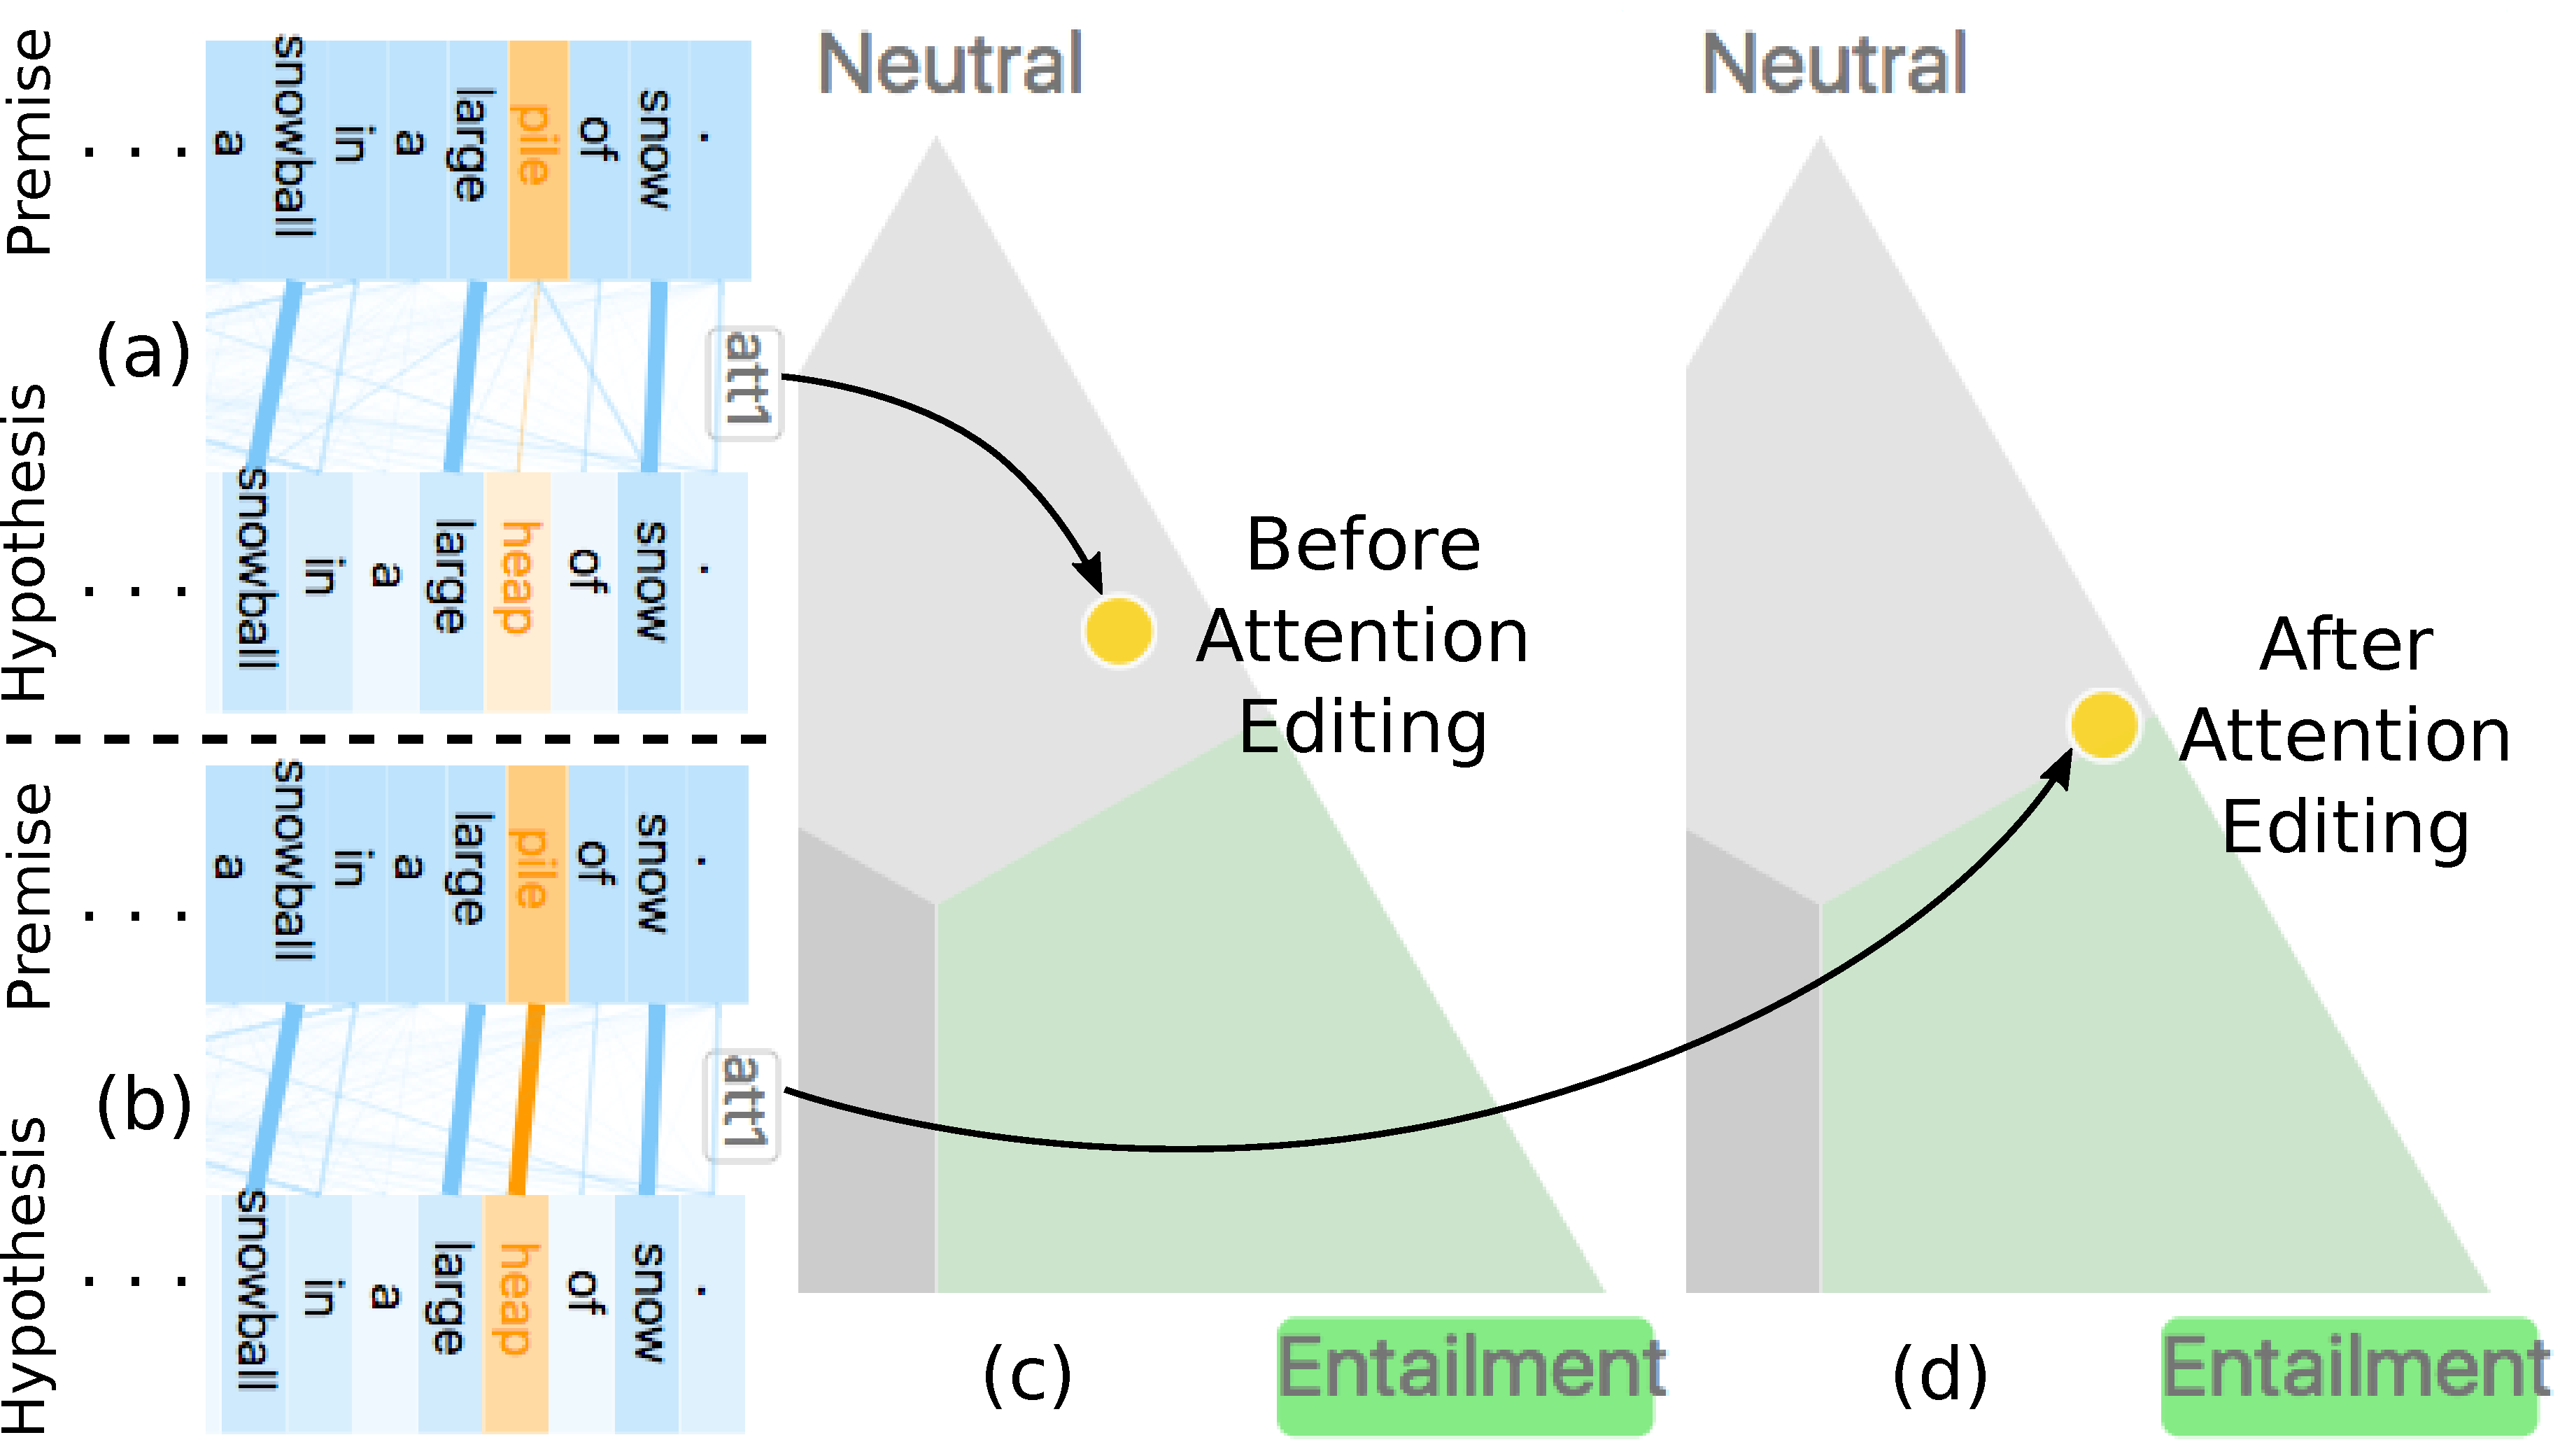
\includegraphics[width=1.0\linewidth]{att2pred}
 \caption{
How attention affect prediction.).
%
}
\label{fig:att2pred}
\end{figure}

\begin{itemize}
\item A very young child in a red plaid coat and pink winter hat makes a snowball in a large pile of snow .
\item A child in a red plaid coat and pink winter hat makes a snowball in a large heap of snow .
\end{itemize}

%Hypothesizing
Interpreting how the model arrive at a prediction is one of the most important goal for the expert driven exploratory analysis.
%

 first step  only essential for evaluating the model performance but also necessary for hypothesizing improvement strategies.
%
The three stages (encoder, attention, classifier) of the model work in synergy to produce the correct prediction.

\begin{figure*}[t]
\centering
\vspace{-2mm}
 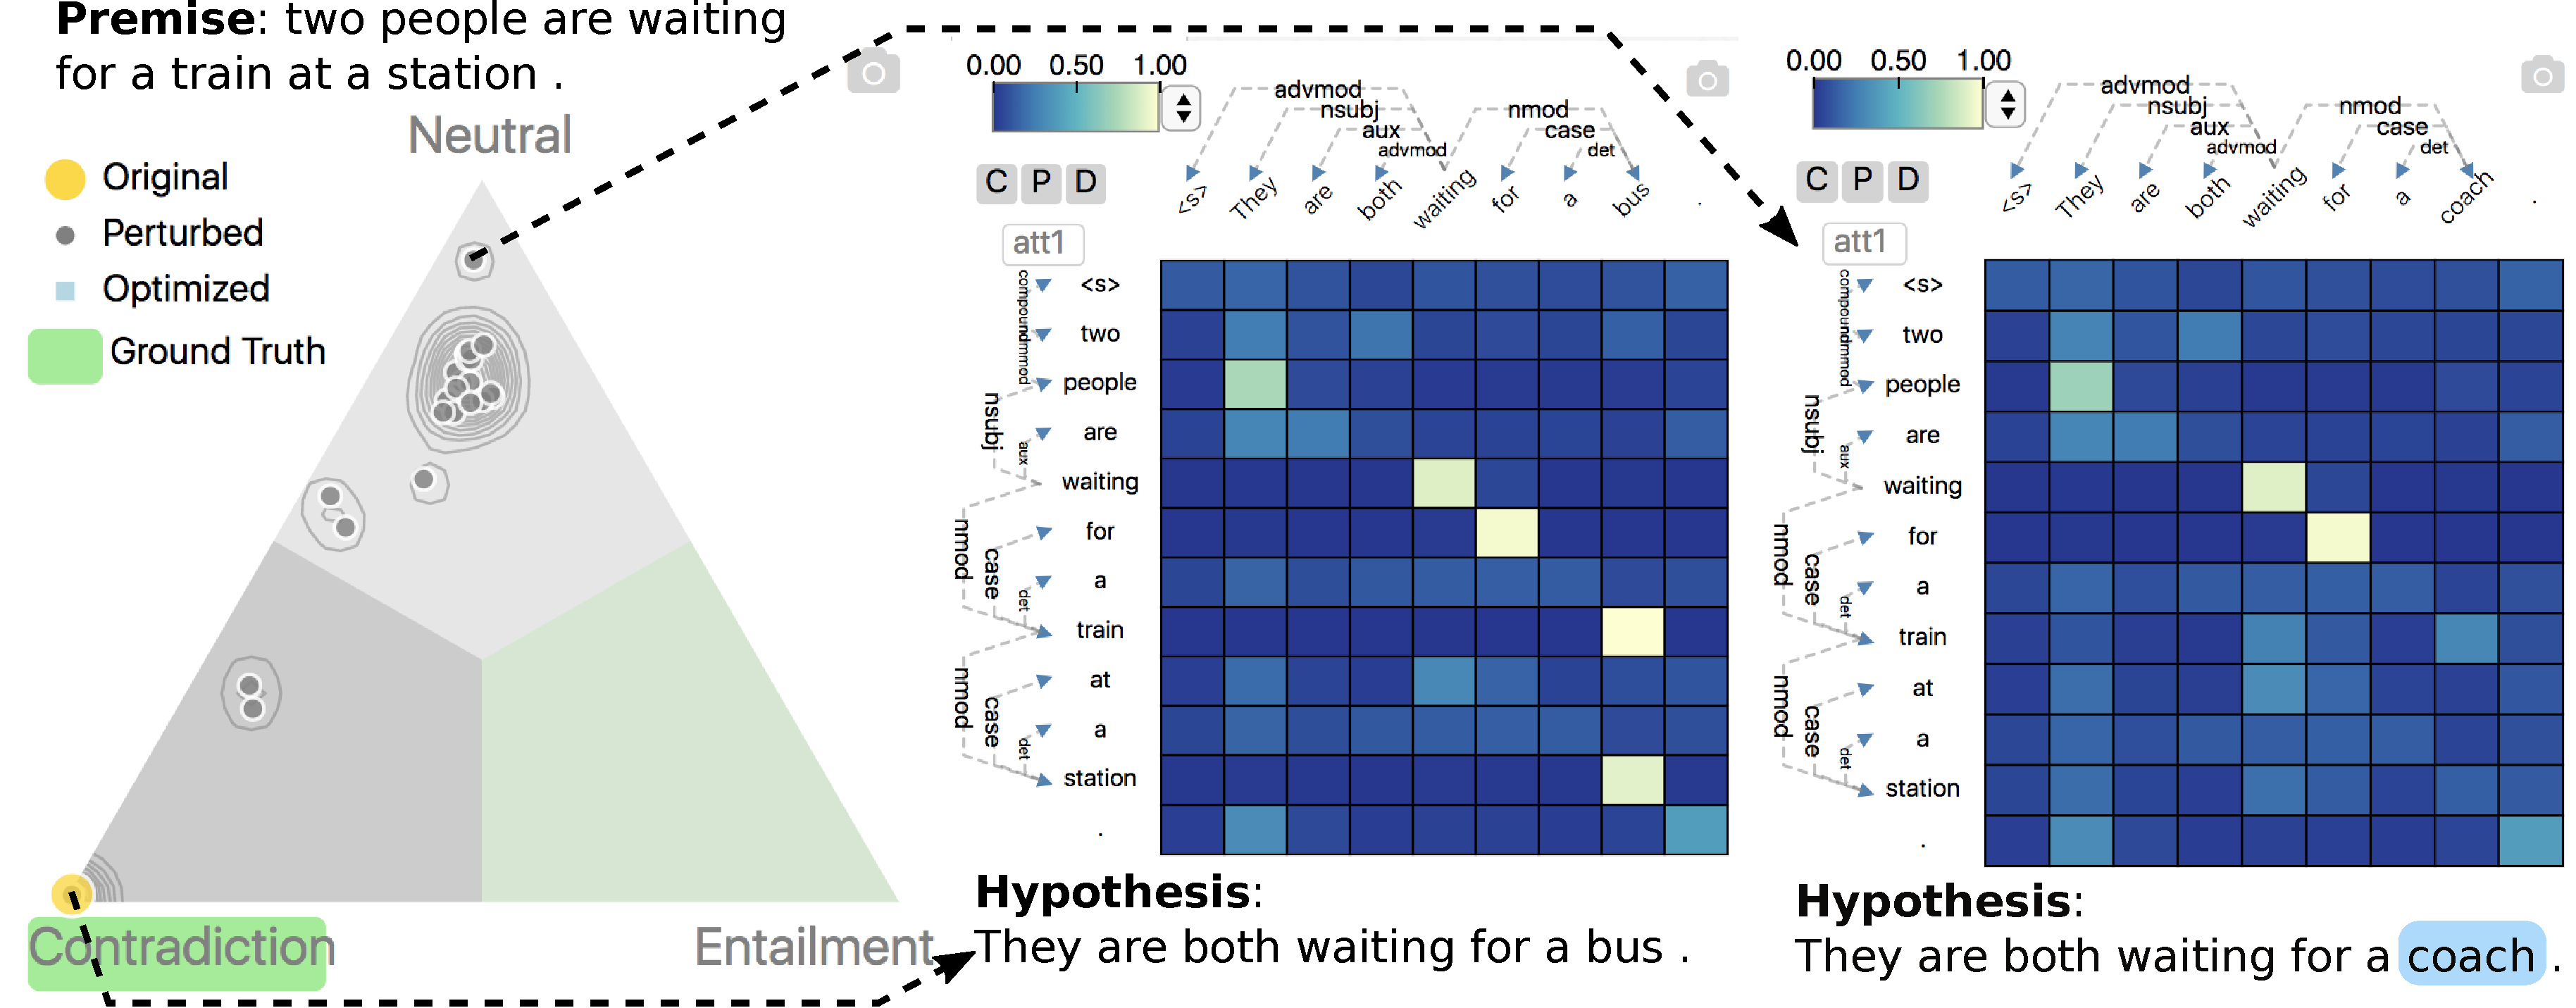
\includegraphics[width=0.9\linewidth]{failledEncoding}
 \caption{
The prediction is failed due to incorrect alignment. For all the failed case, 
 }
\label{fig:failedEncoding}
\end{figure*}


%One of the essential task for can be made in either of these stages.
% \shusen{difference in sensitivity among entail natural and contradict relationships}
% the generate the correct prediction for the wrong reason
Does the model arrived at the correct prediction for the wrong reason?

\subsection{Scenario 3: What Does It Take to Correct a Wrong Prediction?}
In the previous section, we discussed how we can use forward prediction


\subsection{Scenario 4: Explore Relationship Between Grammar and Attention}
Can attention capture grammar structure? Is 

\subsection{Scenario 5: Handcraft Example Analysis}
To test the limitation of the model, domain experts often handcraft ``extreme'' examples (as such the Facebook IPO example discussed in Section~\ref{sec:background}) that they know most model will have a difficult time making correct inference. 
%
%The exploration is just started once the prediction result is examined, 
Often the researchers have a set of "what if..." experiments they would like to run. And dependent on the experiment out come, they like will have new questions to ask and try out the different variations or combinations.
%
In some way, we can think of such a process as a nature blend of all previously discussed scenario, where the domain experts do not necessarily have specific goal in mind, instead focus on probing around and see if they can find anything interesting and out-of-ordinary behaviors in the model.
%
Having an environment, in which the experts can freely modify the words or attention then observe the corresponding changes in other parts of the model pipeline, ensures an streamlined exploration experience that free the users from interruption and grunt work, allow them to focus on more productive activity. 

%\subsection{Is the Prediction Stable?}
%\subsection{Where Are the Mistakes?}
%\subsection{How Attention Affect the Prediction?}
%\subsection{What Does It Take to Change the Prediction?}
%\subsection{Is Attention All You Need?}
